\chapter{Project Structure}
\label{cha:project_structure}
This chapter shows the structure of an project which implements the previously discussed authentication mechanisms.
The aim of this chapter is clarifying the interactions of the components which are needed to not only implement the service-to-service authentication, but also the authentication of the end user.
For the simlicity topics like authorization, key management and user context sharing are not handled in this example.
The visualizations of this chapter are based on the backend of a flea market app.

\section{Preambel Flea Market App}
The flea market app is an Android App written in the programming language Kotlin.
The main features are buying, renting and swapping items.
The user is authenticated using firebase authentication.
He has to present his access token to the Microsoft API Gateway with each request.
The backend of the app is based on the microservice architecture and the microservices are mainly implemented in C\# it actually contains of the following services:
\begin{itemize}
	\item AdService
	\item UserService
	\item ChatService
	\item MediaService
	\item SubscriptionService
	\item ReportService
\end{itemize}
Each service has its own PostgreSQL database.
The services are hosted on Microsoft Azure using docker containers.
Only the AdService and the UserService will be used to show an exemplary example of the communication within the deployment when the discussed authentication mechanisms are implemented.

\section{Exemplary Example}
Figure~\ref{fig:deployment_structure} shows an extract of the previously described backend and visualizes the communication of the needed components.
In this example the user fetches all ads which are in his surrounding.
Therefore the AdService is used to fetch all ads and the UserService is needed to preview some information about the seller.
In this use case the following components are necessary:
\begin{description}
	\item[Android App:] The Android App is the User Interface for the client to access the functionalities of the services.
		The requests sent by the Android App are sent in beyond of the user.
	\item[Firebase Authentication:] The Firebase Authentication service is responsible for validating the access tokens wich are transferred by the users.
		The app also communicates with this service to get an access token, but this is done in an earlier stage.
	\item[API Gateway:] The API Gateway is the only entry point into the deployment.
		Therefore the API Gateway is the only component which directly communicates to the Android App.
	\item[AdService:] The AdService is responsible to manage all ads offered to the user of the app.
	\item[UserService:] The AdService is the service which is responsible for managing the data of the users.
\end{description}

\begin{figure}
	\centering
	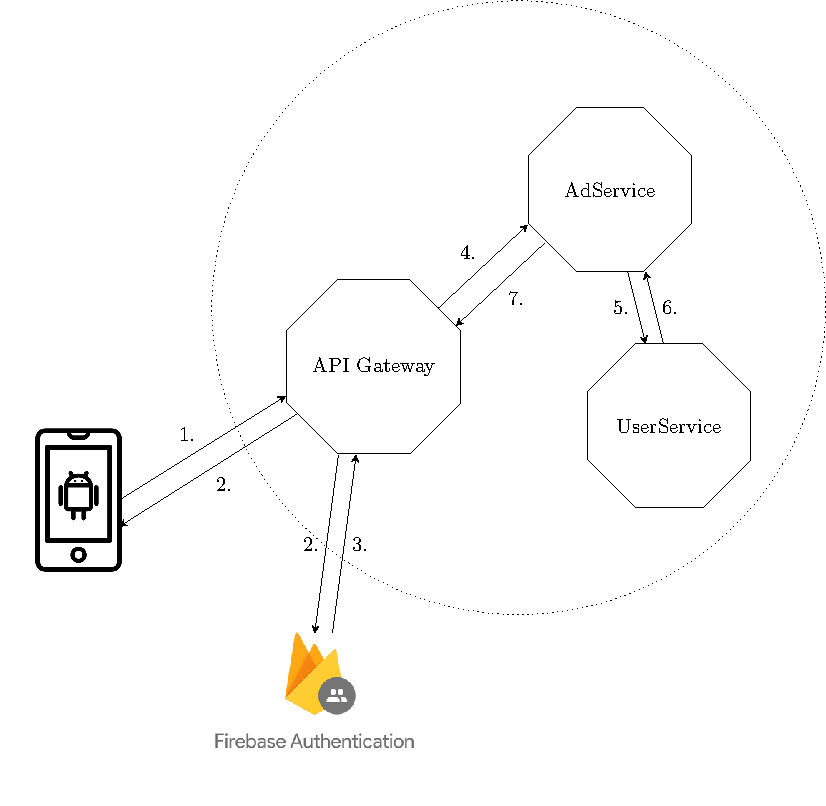
\includegraphics{images/project-structure/TikZ_structure.pdf}
	\caption{Communication among the components of the exemplary example}
	\label{fig:deployment_structure}
\end{figure}

\subsection{Workflow using mTLS}
\begin{enumerate}
	\item[1.] The client sends an API request to the Microsoft API Gateway using the Android App.
		The communication between the API Gateway and the App is secured using HTTPS.
		Therefore the server is authenticated to the client using TLS.
		The client is authenticated to the server by embedding an firebase access token within the Authorization header.
	\item[2.] The API Gateway sends the received token to the Firebase Authentication service to validate it.
		This is defined as a policy within the policy file of the API Gateway.
	\item[3.] The Firebase Authentication service returns the information whether the persented token is valid or not.
	\item[4.] When the client provided a valid access token, the request of the client is forwarded to the \textbf{AdService}.
		The communication between the API Gateway and the \textbf{AdService} is secured using mTLS.
		This means both parties have to present a certificate, signed by a trusted CA.
		Therefore the webserver of the \textbf{AdService} has to be configured to allow or even require Client Certificates.
	\item[5.] After processing the request from the API Gateway the \textbf{AdService} sends a request to the \textbf{UserService} to retrieve the additional information about the owner.
		The communication between the \textbf{UserService} and the \textbf{AdService} is also protected using mTLS, so it has to be configured like the \textbf{AdService}.
		The certificate is appened to the request using a HTTPClient, which is injected to the Controller of the WebService using Dependency Injection.
	\item[6.] When the \textbf{UserService} processed the request, it responds with the expected result.
		The response does not require to perform the authentication again, since TCP connection between the \textbf{AdService} and the \textbf{UserService} is still opened.
	\item[7.] After the \textbf{AdService} processed the response from the \textbf{UserService}, it uses the opened connection with the API Gateway and transfers its response.
	\item[8.] The API Gateway forwards the response from the \textbf{AdService} to the Android App.
		This connection is still secured using TLS and not mTLS.
		The App can now process the response and present the requested information to the user.
\end{enumerate}

\subsection{Workflow using JWT}
The workflow using JWT and the workflow using mTLS are very similar, therefore only the steps which differ between the mechanisms are described again.
\begin{enumerate}
	\item[4.] The request from the client is forwarded to the \textbf{UserService}. 
		Therefore the API Gateway has to create a valid JWT to communicate with the \textbf{UserService}.
		On the Microsoft API Gateway, the logic to create a JWT is implemented as a policy.
		The JWT, which is signed using the private key of the API Gateway is transferred within the Authorization header.
	\item[5.] The \textbf{AdService} has to retrieve additional information from the \textbf{UserService}.
		Now the \textbf{AdService} has to present his JWT to the \textbf{UserService}.
		This is done by using a HTTPClientFactory, which automatically embeds the signed JWT within the Authorization header, when the request is sent.
		If the \textbf{AdService} does not know the certificate of the \textbf{UserService}, it will deny the request and ask the \textbf{AdService} to present its certificate.
		In this case the request is repeated and the certificate of the \textbf{AdService} is transferred during the TLS handshake, like it would be transferred using mTLS.
\end{enumerate}

